\documentclass[11pt,a4paper,titlepage]{beamer}
\usepackage[utf8x]{inputenc}
\usepackage{ucs}
\usepackage{amsmath}
\usepackage{amsfonts}
\usepackage{amssymb}
\usepackage[magyar,english]{babel}
\usepackage{verbatim}
\usepackage{animate}
%\usepackage{movie15}
%\usepackage{animate}
%\usepackage{subfigure}
%\usetheme{Warsaw}
\usecolortheme{crane}
%\usecolortheme{rose}
\beamertemplatenavigationsymbolsempty


\author{Dorottya Cserpán}
\title{Estimation of Single Neuron's
           Current Source Density Distribution
                 by Using Kernel Methods
}
\date{July 1, 2013}
\titlegraphic{\includegraphics[width=2cm]{plots/wignerlogo6.png}\hspace*{2cm}~%
   \includegraphics[width=2cm]{plots/nencki_logo_en.png}\hspace*{2cm}~%
    \includegraphics[width=2cm]{plots/bmelogo.png}}
   

   
\begin{document}



\begin{frame}
\titlepage
\end{frame}

%%%%%%%%%%%%%%%%%%%%%%%%%%%%%%%%%%%%%%%%%%%%%%%%%%%%%%%%%%%%%

%1st frame

\section{Motivation}
 
 \begin{frame}
 \begin{figure}
\includegraphics[height=7cm]{plots/DeutschEtAlFigure2.png}

\end{figure}
\footnote{http://www.eahb.org/DeutschEtAl/DeutschEtAlFigure2.jpg}
 \end{frame}
%%%%%%%%%%%%%%%%%%%%
 \begin{frame}
\begin{columns}
\column{0.5\textwidth}


\begin{figure}
\includegraphics[height=5 cm]{plots/aps_mea.png}
\end{figure}
\column{0.01\textwidth}
\column{0.5\textwidth}

\begin{itemize}
\item Understanding the neural computational mechanism 
\item Information about the inputs
\item Estimation of the ionchannel distribution
\end{itemize} 

Tools:
high density multielectrode arrays
\end{columns}
\begin{block}{Goal}
Method for estimating the current source density distributions of single cells.
\end{block}
\footnote{http://www.apsmea.com/product.html}
\end{frame}

%%%%%%%%%%%%%%%%%%%%%%%%%%%%%%%%%%%%%%%%%%%%%%%%%%%%%%%%%%%%%%%%%%%%%%%%%%%%%%%%
%Idea
%kCSD + sCSD -> ksCSD



\section{The Roots}

\begin{frame}{Current Source Density methods}

Extracellular potentials $\Rightarrow$ Currents
CSD:
\begin{equation}
C(z_j)= - \sigma \frac{\Phi(z_j+h)-2\Phi(z_j)+\Phi(z_j-h)}{h^2}
\end{equation}


\end{frame}


%%%%%%%%%%%%%%%%%%%%%%%%%%%%%%%%%%%%%%%%%%%%%%%%%%%%%%%%%%%%%%%%%%%%%%%%%%%%%%%%
\begin{frame}{CSD}
\begin{figure}
\includegraphics[height=6 cm]{plots/mitzdorf.png}
%\caption{Somogyvari Z.}

\end{figure}

%\begin{equation}
%C(z_j)= - \sigma \frac{\Phi(z_j+h)-2\Phi(z_j)+\Phi(z_j-h)}{h^2}
%\end{equation}
\footnote{Mitzdorf 1985}
\end{frame} 
%%%%%%%%%%%%%%%%%%%%%%%%%%%%%%%%%%%%%%%%%%%%%%%%%%%%%%%%%%%%%%%%%%%%%%%%%%%%%%%%
\begin{frame}{CSD family}
\begin{figure}
\includegraphics[height=6 cm]{plots/csd_family.png}
%\caption{Somogyvari Z.}

\end{figure}

%\footnote{Mitzdorf 1985}
\end{frame} 
%%%%%%%%%%%%%%%%%%%%%%%%%%%%%%%%%%%%%%%%%%%%%%%%%%%%%%%%%%%%%%%%%%%%%%%%%%%%%%%%

\begin{frame}{sCSD}
\begin{columns}
\column{0.5\textwidth}
\begin{figure}
\includegraphics[height=6.5 cm]{plots/Fig1.pdf}
%\caption{Somogyvari Z.}

\end{figure}

\column{0.01\textwidth}
\column{0.4\textwidth}

Point-source equation:
%Poisson-equation \\
%(discrete form):
\begin{equation}
\Phi_{i}(r_i)= \frac{1}{4\pi\sigma} \sum_{j=1}^N \frac{I_j}{|r_i-r_j|}
\end{equation}
Matrix formalism:
\begin{equation}
\mathbf{\Phi}= \mathbf{T} \mathbf{I}
\end{equation}

Inverse solution:
\begin{equation}
\mathbf{I}= \mathbf{T^{-1}} \mathbf{\Phi}
\end{equation}
\end{columns}
\footnote{Somogyvari et al 2012}
% \textit{Localization of single-cell current sources based on extracellular potential patterns: the spike CSD method.}, Eur J Neurosci 2012.}
\end{frame}
%%%%%%%%%%%%%%%%%%%%%%%%%%%%%%%%%%%%%%%%%%%%%%%%%%%%%%%%%%%%%%%%%%%%%%%%%%%%%%%%
\begin{frame}{kCSD}
\begin{figure}
\includegraphics[height=3 cm]{plots/kCSD.png}
%\caption{Somogyvari Z.}

\end{figure}
\begin{itemize}
\item kernel method
\item number of current sources $>$ number of electrodes
\end{itemize}


\footnote{Potworowski et al. 2012}
\end{frame}




%%%%FRAME
%Assumptions & model


\section{The skCSD method}
\subsection{Theoretical Issues}
\begin{frame}{skCSD}
%This method is based on the work of Wójcik et al (2012).


$\tilde{b}$:  source function - the activity of a neural segment

\begin{itemize}
%\item step function
\item Gaussian function
\begin{equation}
\tilde{b}_i (t') = e^{- \frac{(t' - t_i)^2}{R^2}}
\end{equation}

\item Cosinus function
\begin{equation}
\tilde{b}_i (t') =\frac{cos(|t' - t_i|) \pi}{R} ,\quad \text{if $|t' - t_i|<R$}
 %\tilde{b}_i (t') = \left\{ 
  % \begin{array}{l l}
   %  \frac{cos(|t' - t_i|) \pi}{R} & \quad \text{if |t' - t_i|<R}\\
   % 0 & \quad \text{else}
   %\end{array} 
\end{equation}
%\tilde{b}_i (t') =\frac{cos(|t' - t_i|) \pi}{R}

\end{itemize} 

Current density at $\textbf{x}$:
\begin{equation}
C (\textbf{x})= \sum_{j=i}^M a_j \tilde{b}_j(\textbf{x})
\end{equation}



%\begin{block}{Questions}
%What kind of base function to use? \\ How to choose R?
%\end{block}



\end{frame}

\begin{frame}

The extracellular potential generated by the ith source:
\begin{equation}
b_i (x,y,z)= A \tilde{b}_i (t') 
\end{equation}
\begin{equation}
b_i (x,y,z)= \frac{1}{4 \pi \sigma} \int
\frac{ \tilde{b}_i (t')}{\sqrt{(x-x'(t))^2+(y-y'(t))^2+(z-z'(t))^2}} dt'
\end{equation}


\begin{equation}
\Phi (\textbf{x})= \sum_{i=1}^M a_i b_i(\textbf{x})
\end{equation}


%\begin{columns}
%\column{0.45\textwidth}
%\begin{figure}
%\includegraphics[width=3.5 cm]{pics/integration.png}

%\end{figure}

%\column{0.45\textwidth}

%\begin{block}{Questions}
%Numerical integration? \\ How to choose R?
%\end{block}
%\end{columns}
\end{frame}

%%%%%%%%%%%%%%%%%%%%%%%%%%%%%%%%%%%%%%%%%%%%%%%%%%%%%%%%%%%%%%%%%%%%%%%%%%%%%%%%
\begin{frame}
%The detailed derivation of this method can be found in the \cite{DanielW}. reference, due to the length limitation it's not detailed here.
To determine the CSD distribution in arbitrary positions($x$), the following kernel functions were introduced:

%Let's create a matrix $\tilde{B}$ from the $\tilde{b}_i$ functions, where the rows correspond to the $i$th functions and the columns for all the locations of the sources, so that the value $\tilde{B}_{ij}$ is $\tilde{b}_i (\textbf{x}_j)$
\begin{equation}
K(\textbf{x}_k,\textbf{x}_l)= \sum_{i=1}^M b_i (\textbf{x}_k) b_i (\textbf{x}_l) = B_k^T B_l
\end{equation} 
 
\begin{equation}
\tilde{K}(\textbf{x}_k,\textbf{y}_l)= \sum_{j=1}^M b_ (\textbf{x}_k) \tilde{b}_j (\textbf{y}_l)  = B_k^T \tilde{B}_l
\end{equation} 
 
Using the simulated or measured extracellular potentials ($V$) and assuming $\tilde{K}$ is invertible the solution for $C$ is straightforward.
 \begin{equation}
 C(\textbf{x})=\tilde{\textbf{K}}^T(\textbf{x})  
 \tilde{\textbf{K}}^{-1} \textbf{V}
 \end{equation}


\end{frame}

%%%%%%%%%%%%%%%%%%%%%%%%%%%%%%%%%%%%%%%%%%%%%%%%%%%%%%%%%%%%%%%%%%%%%%%%%%%%%%%%
\subsection{Practical issues}

\begin{frame}{Usually neurons have more, than 1 branch :(}
\begin{columns}
\column{0.5\textwidth}
\begin{figure}
\includegraphics[height=6 cm]{plots/cellmorph.png}
\end{figure}
\column{0.1\textwidth}
\column{0.4\textwidth}
How to handle the branching?
\begin{itemize}
\item branches independent
\item connect the branches
\end{itemize}
\end{columns}
\footnote{$http://neuromorpho.org/neuroMorpho/neuron_info.jsp?
neuron_name=03a_pyramidal9aFI$ \
Allman et al 2006}
\end{frame}


%%%%%%%%%%%%%%%%%%%%%%%%%%%%%%%%%%%%%%%%%%%%%%%%%%%%%%%%%%%%%%%%%%%%%%%%%%%%%%%%
\begin{frame}{Usually branches are not straight :((}
\begin{columns}
\column{0.5\textwidth}
\begin{figure}
\includegraphics[height=6 cm]{plots/9thbranch.png}
\end{figure}
\column{0.1\textwidth}
\column{0.4\textwidth}
How to handle?
\begin{itemize}
\item fit a curve
%\item connect the branches
\item position given by parameter $t$
\end{itemize}
\end{columns}
\end{frame}


%%%%%%%%%%%%%%%%%%%%%%%%%%%%%%%%%%%%%%%%%%%%%%%%%%%%%%%%%%%%%%%%%%%%%%%%%%%%%%%%
\begin{frame}{Lots of parameters :(((}
\begin{columns}
\column{0.5\textwidth}
Parameters of the method:
\begin{itemize}
\item type of basis function
\item number of basis function
\item width of basis function
\end{itemize}
%\column{0.1\textwidth}
\column{0.4\textwidth}
Parameters of the test simulations:
\begin{itemize}
\item neuron morphology
\item inputs
\item cell to electrode distance
\item position of the electrode (1D, 2D, 3D)

\end{itemize}
\end{columns}

\end{frame}



%%%%%%%%%%%%%%%%%%%%%%%%%%%%%%%%%%%%%%%%%%%%%%%%%%%%%%%%%%%%%%%%%%%%%%%%%%%%%%%%


%%%%%%%%%%%%%%%%%%%%%%%%%%%%%%%%%%%%%%%%%%%%%%%%%%%%%%%%%%%%%%%%%%%%%%%%%%%%%%%%

\begin{frame}
\begin{figure}
\includegraphics[height=8 cm]{plots/flow.png}
\end{figure}

\end{frame}

%%%%%%%%%%%%%%%%%%%%%%%%%%%%%%%%%%%%%%%%%%%%%%%%%%%%%%%%%%%%%%%%%%%%%%%%%%%%%%%%
\section{Simulations}
\begin{frame}{Ballstick neuron}
\begin{columns}
\column{0.5\textwidth}
\begin{figure}
\includegraphics[height=5cm]{plots/bssetup.png}

\end{figure}
%%%%%%%%%%%%%%%%%%%%%%%%%%%%%%%%%%%%%%%%%%%%%%%%%%%%%%%%%%%%%%%%%%%%%%%%%%%%%%%%
%\column{0.1\textwidth}
\column{0.5\textwidth}
\begin{figure}
\includegraphics[height=3 cm]{plots/bsLFP.png}
\end{figure}

\end{columns}
\end{frame}

\begin{frame}{ksCSD for ballstick neuron}
\begin{figure}
\includegraphics[height=8 cm]{plots/bsCSD.png}
\end{figure}

\end{frame}

%%%%%%%%%%%%%%%%%%%%%%%%%%%%%%%%%%%%%%%%%%%%%%%%%%%%%%%%%%%%%%%%%%%%%%%%%%%%%%%%
\begin{frame}{Ballstick neuron}

\begin{figure}
\includegraphics[height=5.5cm]{plots/error_Rtest_cos_patt3_12_el_both.png}
\end{figure}
\end{frame}

\begin{frame}{Ballstick neuron}

\begin{figure}
\includegraphics[height=5.5cm]{plots/error_Rtest_cos_patt13_22_el_both.png}
\end{figure}
\end{frame}
%%%%%%%%%%%%%%%%%%%%%%%%%%%%%%%%%%%%%%%%%%%%%%%%%%%%%%%%%%%%%%%%%%%%%%%%%%%%%%%%
\section{Simulations}
\begin{frame}{Complex morphology}
\begin{figure}
\includegraphics[height=6.8 cm]{plots/lfpy_setup.pdf}
\end{figure}

\end{frame}


%%%%%%%%%%%%%%%%%%%%%%%%%%%%%%%%%%%%%%%%%%%%%%%%%%%%%%%%%%%%%%%%%%%%%%%%%%%%%%%%

\begin{frame}
\begin{figure}
\includegraphics[height=6.8 cm]{plots/moprhology3d.png}
\end{figure}

\end{frame}

%%%%%%%%%%%%%%%%%%%%%%%%%%%%%%%%%%%%%%%%%%%%%%%%%%%%%%%%%%%%%%%%%%%%%%%%%%%%%%%%
\section{Results}
%%%%%%%%%%%%%%%%%%%%%%%%%%%%%%%%%%%%%%%%%%%%%%%%%%%%%%%%%%%%%%%%%%%%%%%%%%%%%%%%



%%%%%%%%%%%%%%%%%%%%%%%%%%%%%%%%%%%%%%%%%%%%%%%%%%%%%%%%%%%%%%%%%%%%%%%%%%%%%%%%

\begin{frame}
\begin{figure}
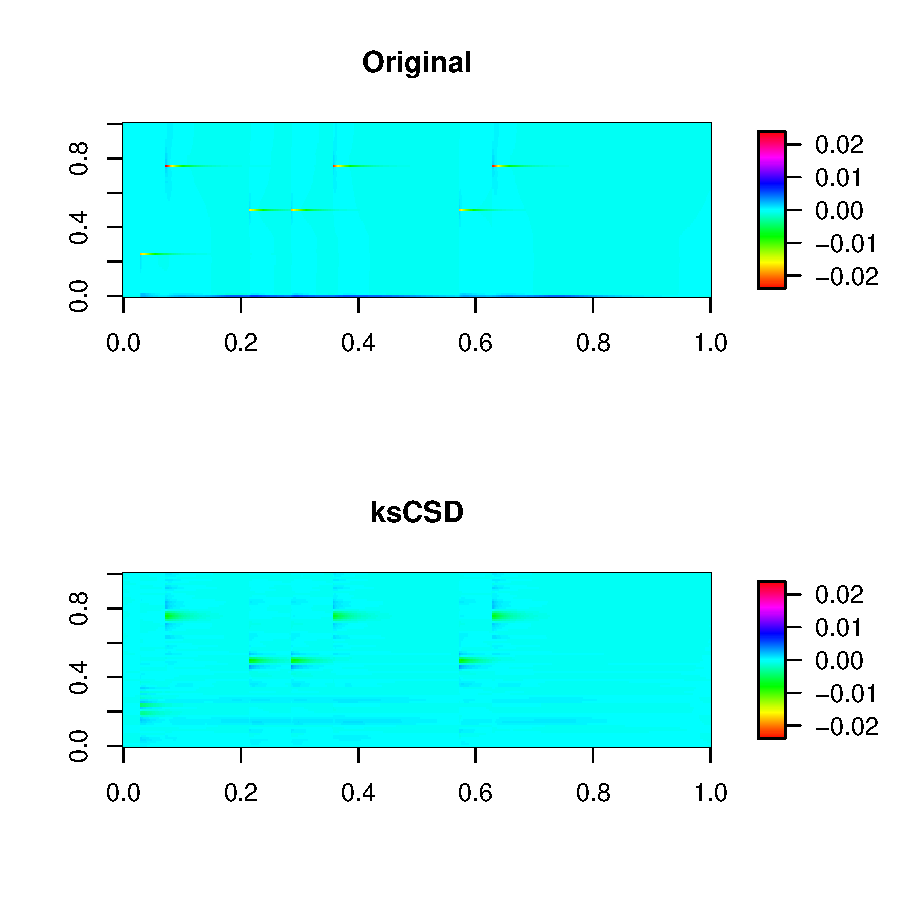
\includegraphics[height=9 cm]{plots/pl-kCSDplot.pdf}
\end{figure}

\end{frame}



%%%%%%%%%%%%%%%%%%%%%%%%%%%%%%%%%%%%%%%%%%%%%%%%%%%%%%%%%%%%%%%%%%%%%%%%%%%%%%%%

\begin{frame}
\begin{figure}
\includegraphics[height=8 cm]{plots/colourpoints.png}
\end{figure}

\end{frame}

%%%%%%%%%%%%%%%%%%%%%%%%%%%%%%%%%%%%%%%%%%%%%%%%%%%%%%%%%%%%%%%%%%%%%%%%%%%%%%%%


\begin{frame}{Future plans}
\begin{itemize}
\item Run more test simulations
\item Make the program usable also for others (GUI)
\item Test the method on experimental data 
\end{itemize}

\end{frame}

%%%%%%%%%%%%%%%%%%%%%%%%%%%%%%%%%%%%%%%%%%%%%%%%%%%%%%%%%%%%%%%%%%%%%%%%%%%%%%%%


\begin{frame}
\begin{center}

{\Large Thanks for the attention!}
\end{center}
\end{frame}



%%%%%%%%%%%%%%%%%%%%%%%%%%%%%%%%%%%%%%%%%%%%%%%%%%%%%%%%%%%%%%%%%%%%%%%%%%%%%%%%
\begin{frame}{Which is the best set of parameters?}
\begin{equation}
e= \frac{\sum\limits_{t,i} |C_{skCSD}-C_o|}{\sum\limits_{t,i}|C_o|}
\end{equation}
\end{frame}






\end{document}